%  !TeX  root  =  user_guide.tex

\section{Быстрая печать}\label{quickprint}

% when the revision of a section has been finalized,
% comment out the following line:
% \updatedisclaimer

Модуль \toolbtntwo{quick_print}{Быстрая печать} позволяет быстро, с
минимальными усилиями экспортировать текущую карту в формат PDF. Необходимо
задать только заголовок карты, имя карты и размер страницы
(см. Рисунок~\ref{fig:quickprint}). Если нужен больший контроль над
результатом, пожалуйста, используйте Компоновщик карты, описанный в
Разделе~\ref{label_printcomposer}.

\begin{figure}[ht]
   \centering
   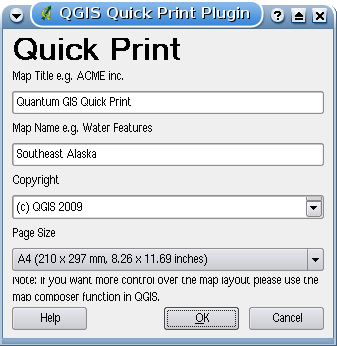
\includegraphics[clip=true, width=6cm]{quick_print_dialog}
   \caption{Модуль Быстрой печати \wincaption}\label{fig:quickprint}
\end{figure}

\begin{figure}[ht]
   \centering
   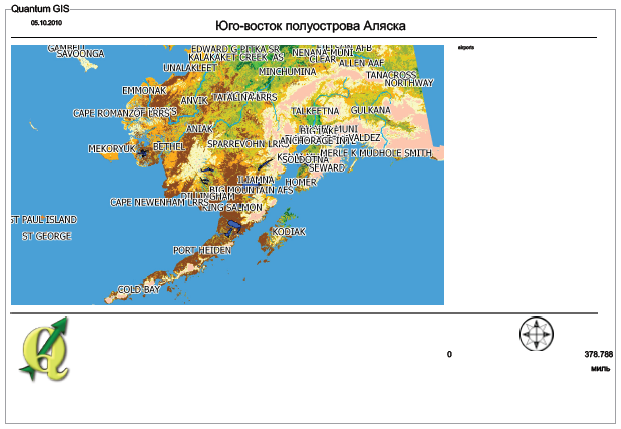
\includegraphics[clip=true, width=9cm]{quick_print_result}
   \caption{Результат работы Модуля Быстрой печати при использовании демонстрационного
   набора данных alaska и размера страницы DIN A4 \wincaption}\label{fig:quickprint_result}
\end{figure}

\FloatBarrier
